\documentclass[border=10pt]{standalone}
\usepackage{pgfplots}
\pgfplotsset{compat=1.18}
\begin{document}
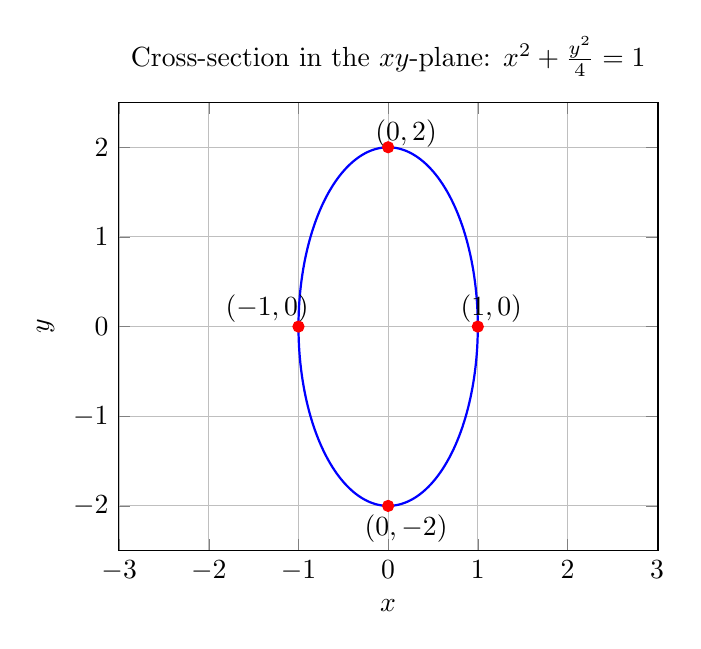
\begin{tikzpicture}
\begin{axis}[
    xlabel={$x$}, ylabel={$y$},
    xmin=-2, xmax=2, ymin=-2.5, ymax=2.5,
    axis equal,
    grid=major,
    title={Cross-section in the $xy$-plane: $x^2+\frac{y^2}{4}=1$},
    samples=200
]
\addplot[blue, thick, domain=0:360] ({cos(x)}, {2*sin(x)});
\addplot[only marks, mark=*, red] coordinates {(1,0) (-1,0) (0,2) (0,-2)};
\node at (axis cs:1.15,0.2) {$(1,0)$};
\node at (axis cs:-1.35,0.2) {$(-1,0)$};
\node at (axis cs:0.2,2.15) {$(0,2)$};
\node at (axis cs:0.2,-2.25) {$(0,-2)$};
\end{axis}
\end{tikzpicture}
\end{document}
